% ----------------------------------------------------
% Theory
% ----------------------------------------------------
%\documentclass[class=report,11pt,crop=false]{standalone}
%% Page geometry
\usepackage[a4paper,margin=20mm,top=25mm,bottom=25mm]{geometry}

% Font choice
\usepackage{lmodern}

% Use IEEE bibliography style
\bibliographystyle{IEEEtran}

% Line spacing
\usepackage{setspace}
\setstretch{1.20}

% Allows us to create dummy text
\usepackage{lipsum}

% Ensure UTF8 encoding
\usepackage[utf8]{inputenc}

% Language standard (not too important)
\usepackage[english]{babel}

% Skip a line in between paragraphs
\usepackage{parskip}

% For the creation of dummy text
\usepackage{blindtext}

% Math
\usepackage{amsmath}

% Header & Footer stuff
\usepackage{fancyhdr}
\pagestyle{fancy}
\fancyhead{}
\fancyhead[R]{\nouppercase{\rightmark}}
\fancyfoot{}
\fancyfoot[C]{\thepage}
\renewcommand{\headrulewidth}{0.0pt}
\renewcommand{\footrulewidth}{0.0pt}
\setlength{\headheight}{13.6pt}

% Epigraphs
\usepackage{epigraph}
\setlength\epigraphrule{0pt}
\setlength{\epigraphwidth}{0.65\textwidth}

% Colour
\usepackage{color}
\usepackage[dvipsnames]{xcolor}

% Hyperlinks & References
\usepackage{hyperref}
\definecolor{linkColour}{RGB}{77,71,179}
\hypersetup{
    colorlinks=true,
    linkcolor=linkColour,
    filecolor=linkColour,
    urlcolor=linkColour,
    citecolor=linkColour,
}
\urlstyle{same}

% Automatically correct front-side quotes
\usepackage[autostyle=false, style=ukenglish]{csquotes}
\MakeOuterQuote{"}

% Graphics
\usepackage{graphicx}
\graphicspath{{Images/}{../Images/}}
\usepackage{makecell}
\usepackage{transparent}

% SI units
\usepackage{siunitx}

% Microtype goodness
\usepackage{microtype}

% Listings
\usepackage[T1]{fontenc}
\usepackage{listings}
\usepackage[scaled=0.8]{DejaVuSansMono}

% Custom colours for listings
\definecolor{backgroundColour}{RGB}{250,250,250}
\definecolor{commentColour}{RGB}{73, 175, 102}
\definecolor{identifierColour}{RGB}{196, 19, 66}
\definecolor{stringColour}{RGB}{252, 156, 30}
\definecolor{keywordColour}{RGB}{50, 38, 224}
\definecolor{lineNumbersColour}{RGB}{127,127,127}
\lstset{
  language=Matlab,
  captionpos=b,
  aboveskip=15pt,belowskip=10pt,
  backgroundcolor=\color{backgroundColour},
  basicstyle=\ttfamily,%\footnotesize,        % the size of the fonts that are used for the code
  breakatwhitespace=false,         % sets if automatic breaks should only happen at whitespace
  breaklines=true,                 % sets automatic line breaking
  postbreak=\mbox{\textcolor{red}{$\hookrightarrow$}\space},
  commentstyle=\color{commentColour},    % comment style
  identifierstyle=\color{identifierColour},
  stringstyle=\color{stringColour},
   keywordstyle=\color{keywordColour},       % keyword style
  %escapeinside={\%*}{*)},          % if you want to add LaTeX within your code
  extendedchars=true,              % lets you use non-ASCII characters; for 8-bits encodings only, does not work with UTF-8
  frame=single,	                   % adds a frame around the code
  keepspaces=true,                 % keeps spaces in text, useful for keeping indentation of code (possibly needs columns=flexible)
  morekeywords={*,...},            % if you want to add more keywords to the set
  numbers=left,                    % where to put the line-numbers; possible values are (none, left, right)
  numbersep=5pt,                   % how far the line-numbers are from the code
  numberstyle=\tiny\color{lineNumbersColour}, % the style that is used for the line-numbers
  rulecolor=\color{black},         % if not set, the frame-color may be changed on line-breaks within not-black text (e.g. comments (green here))
  showspaces=false,                % show spaces everywhere adding particular underscores; it overrides 'showstringspaces'
  showstringspaces=false,          % underline spaces within strings only
  showtabs=false,                  % show tabs within strings adding particular underscores
  stepnumber=1,                    % the step between two line-numbers. If it's 1, each line will be numbered
  tabsize=2,	                   % sets default tabsize to 2 spaces
  %title=\lstname                   % show the filename of files included with \lstinputlisting; also try caption instead of title
}

% Caption stuff
\usepackage[hypcap=true, justification=centering]{caption}
\usepackage{subcaption}

% Glossary package
% \usepackage[acronym]{glossaries}
\usepackage{glossaries-extra}
\setabbreviationstyle[acronym]{long-short}

% For Proofs & Theorems
\usepackage{amsthm}

% Maths symbols
\usepackage{amssymb}
\usepackage{mathrsfs}
\usepackage{mathtools}

% For algorithms
\usepackage[]{algorithm2e}

% Spacing stuff
\setlength{\abovecaptionskip}{5pt plus 3pt minus 2pt}
\setlength{\belowcaptionskip}{5pt plus 3pt minus 2pt}
\setlength{\textfloatsep}{10pt plus 3pt minus 2pt}
\setlength{\intextsep}{15pt plus 3pt minus 2pt}

% For aligning footnotes at bottom of page, instead of hugging text
\usepackage[bottom]{footmisc}

% Add LoF, Bib, etc. to ToC
\usepackage[nottoc]{tocbibind}

% SI
\usepackage{siunitx}

% For removing some whitespace in Chapter headings etc
\usepackage{etoolbox}
\makeatletter
\patchcmd{\@makechapterhead}{\vspace*{50\p@}}{\vspace*{-10pt}}{}{}%
\patchcmd{\@makeschapterhead}{\vspace*{50\p@}}{\vspace*{-10pt}}{}{}%
\makeatother
%
\newacronym{radar}{RADAR}{Radio Detection and Ranging}

%\begin{document}
\ifstandalone
\tableofcontents
\fi
% ----------------------------------------------------
\chapter{Testing \& Results \label{ch:results}}
%\epigraph{Nobody can build you the bridge over which you must cross the river of life, nobody but you alone.}%
%    {\emph{---Friedrich Nietzsche}}
\vspace{0.5cm}
% ----------------------------------------------------



\section{Test setup \& Equipment}

    \begin{figure}[H]
    \centering
    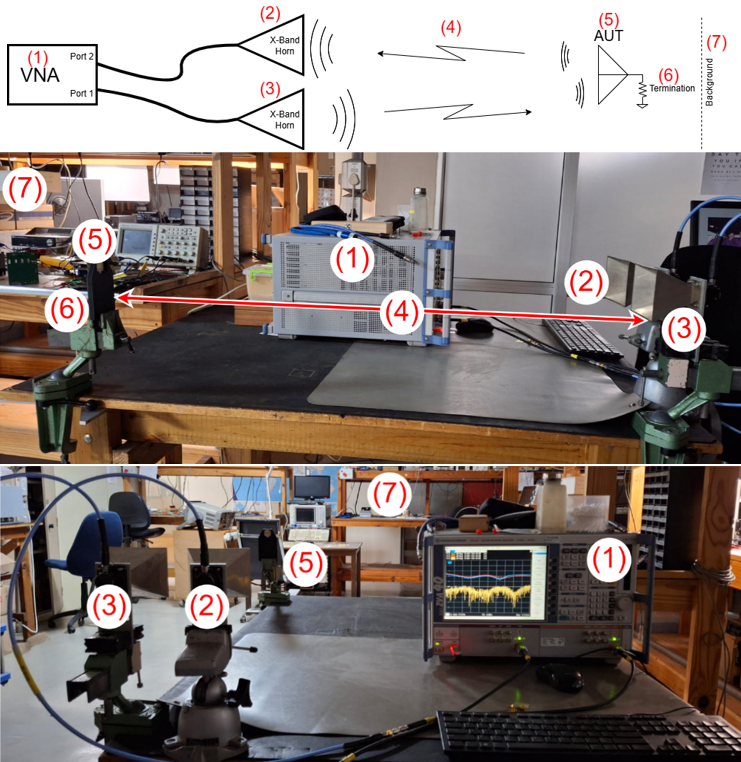
\includegraphics[width=0.9\linewidth]{Figures/chp4_setup.png}
    \caption{Test Setup.}
    \label{fig:chp4_setup}
    \end{figure}

Figure \ref{fig:chp4_setup} show the labelled block diagram of the test setup along with the labelled physical test setup used for all the measurements in this section.
\begin{enumerate}
    \item The Rohde \& Schwarz ZVA 40 VNA was used. This a 2 port \(10MHz-40GHz\) VNA.
    \item This is one of two identical reflective covered injection moulded X-band horn antennae. This antenna acts as the transmit antenna. Since the signal measured will be extremely small in magnitude a horn antenna was chosen for the high gain and directivity.
    \item This is the other X-band horn antennae that was used as the receive antenna. The center of the aperture of the horn antennae are aligned.
    \item The AUT must be placed in the Farfield region of all the antennae. Since the X-Band horn antenna have the largest aperture, the min distance will be the were the Farfield of the horn antennae start.
    \item The AUT is placed in the design bracket and the bracket does not move for a set of measurements. The bracket is designed to keep the position of the AUT fixed when swapping the antennae. The center of the patch is aligned with the aperture of the horn antennae.
    \item Instead of changing the termination of each measurement, three different antennae are used with a termination connect. See figure \ref{fig:chp4_AUTs} below.
    \item Since the measurement were done in the laboratory of a Radar company, the measurements were done after hours and all other equipment in the laboratory was switched off. 
\end{enumerate}

    \begin{figure}[H]
    \centering
    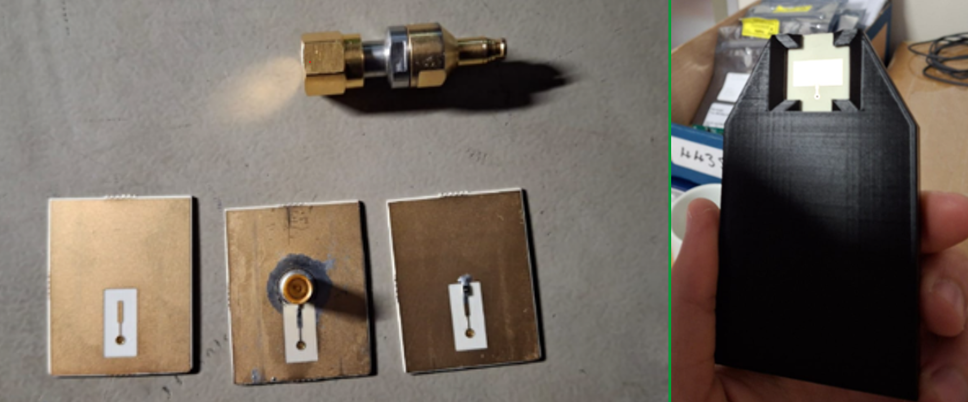
\includegraphics[width=0.5\linewidth]{Figures/chp4_AUTs.png}
    \caption{Three different AUT used during testing.}
    \label{fig:chp4_AUTs}
    \end{figure}

Before the investigation can be done with the design patch antenna, the antenna design must first be verified. The measured return loss of the connectorized antenna is seen in figure \ref{fig:chp4_AUT_S11} below. Although the deep null of -40dB is not seen, the return loss of -19.5dB at the center frequency is still a well-designed antenna. The center frequency is also lower by a 98MHz which equates to a difference in antenna width of $\pm$200um or antenna length of $\pm$90um according to CST studio simulations.

    \begin{figure}[H]
    \centering
    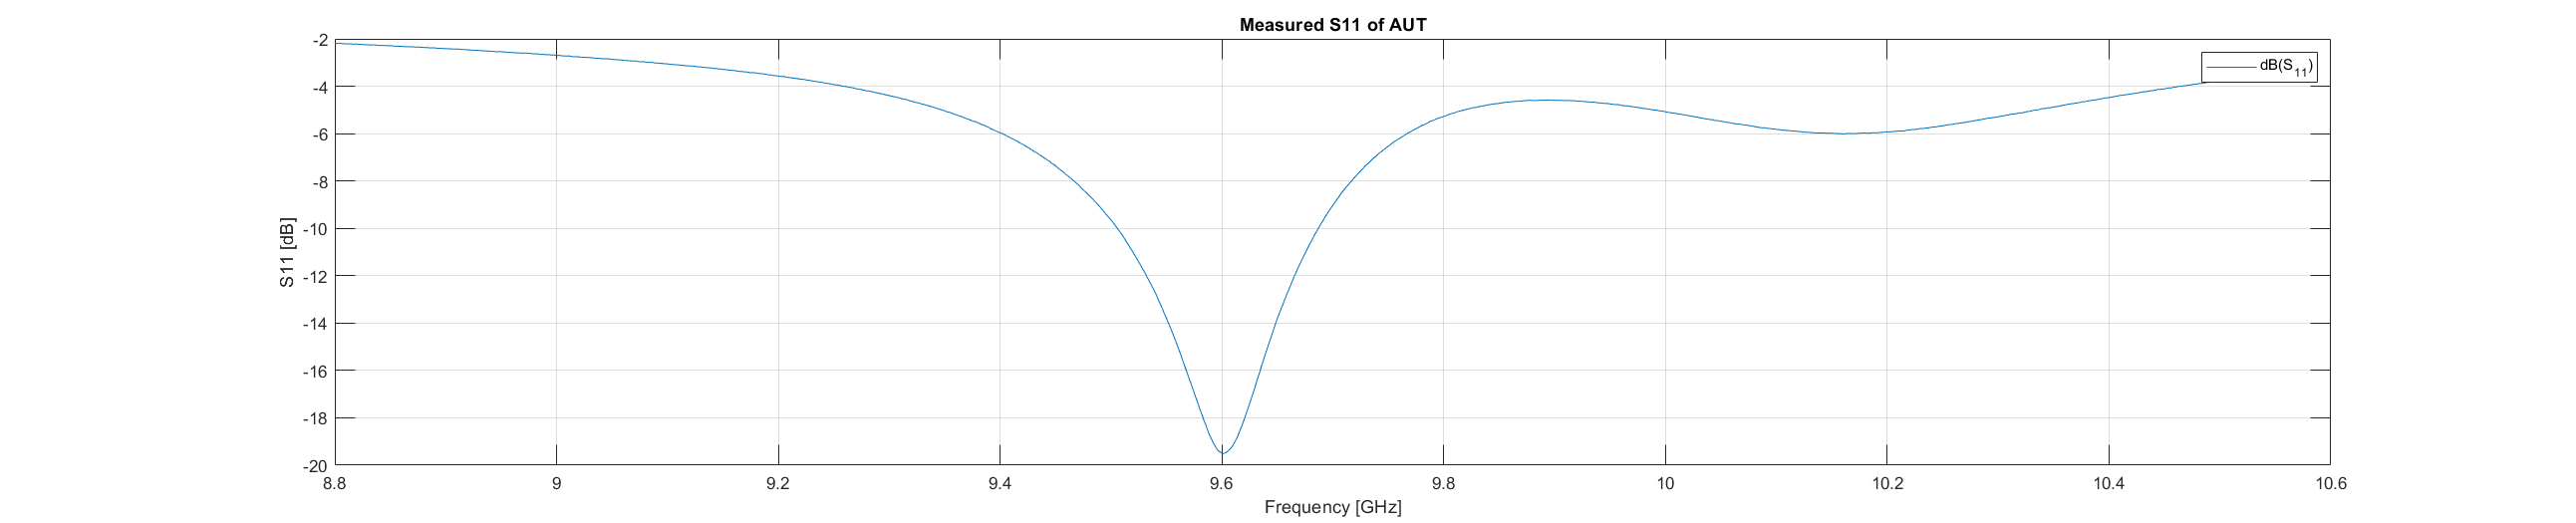
\includegraphics[width=0.99\linewidth]{Figures/chp4_AUT_S11.png}
    \caption{Measured return loss of the design patch (AUT).}
    \label{fig:chp4_AUT_S11}
    \end{figure}

\section{Results}
The test procedure involves moving the AUT into the Farfield of the X-Band horn antennae then doing three separate measurements. One with the open load antenna, a second with the short-circuited antenna a third with the SMP antenna with a SMA 50Ω termination connected to it. The Farfield region of the X-Band horn is calculated below as 584mm. At set of measurements were done with the AUT 600mm, 700mm, 800mm and 900mm away from the horn antennae.
    \[R_{ff}=\frac{2D^2}{\lambda}=\frac{2{(95mm)}^2}{30.91mm}=584mm\]

Analyzing the raw \(S_{21}\) data for the 800mm measurements, as seen in figure \ref{fig:chp4_Raw_results} below, the measured magnitude is the same for both the short circuit and the open circuit AUT. The only visible difference is near the center frequency of the AUT. The same is seen in figure \ref{fig:chp4_Raw_results} for the measured \(S_{21}\) phases of the short circuit and open circuit AUT. 

    \begin{figure}[H]
    \centering
    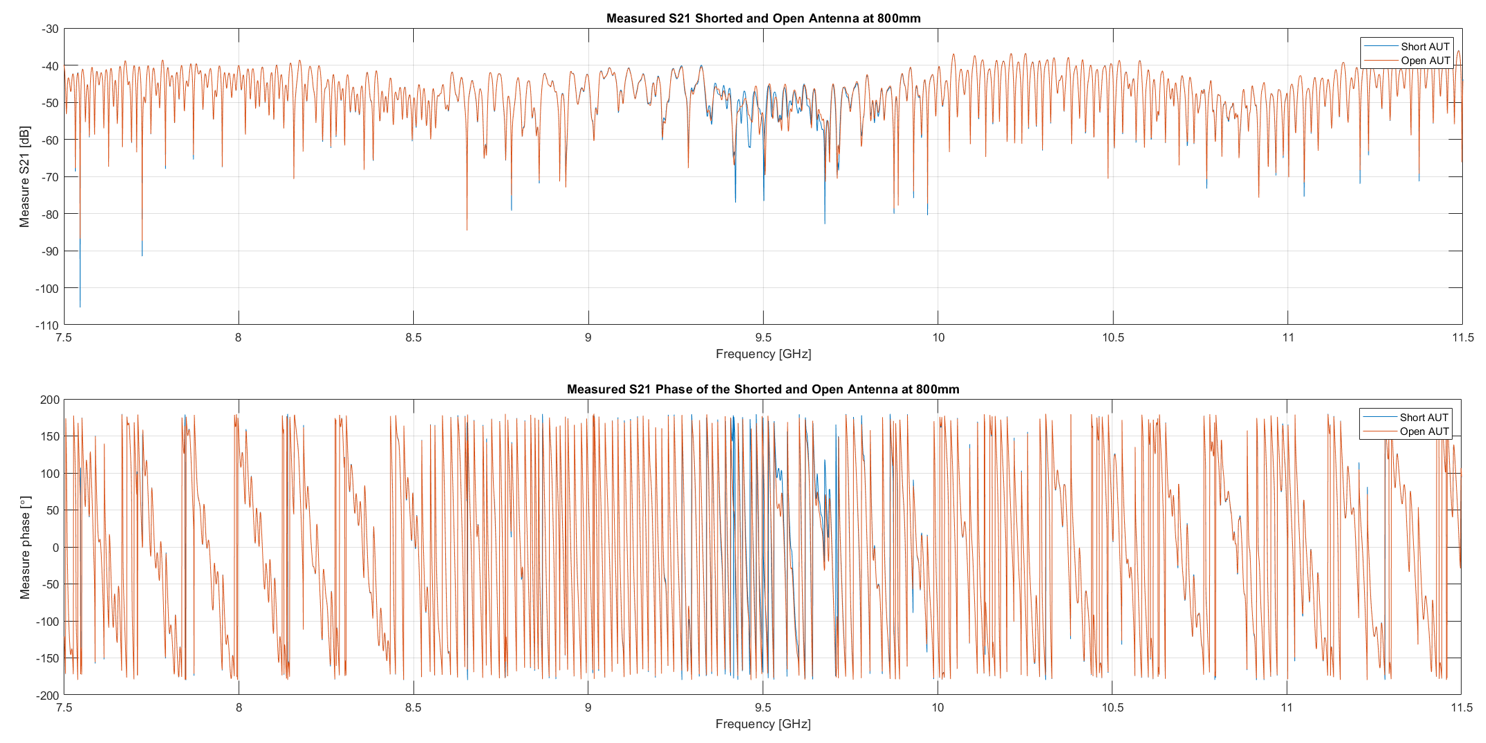
\includegraphics[width=0.99\linewidth]{Figures/chp4_Raw_results.png}
    \caption{Measured \(S_{21}\) magnitude \& phase.}
    \label{fig:chp4_Raw_results}
    \end{figure}

Figure \ref{fig:chp4_Raw_difference_results} below show the zoomed-in view of figure \ref{fig:chp4_Raw_results} as well as the phase difference between the short circuit and open circuit AUT of the measured and unprocessed \(S_{21}\). It is clear that the maximum difference occurs close to the center frequency, which is the opposite response that is aimed for. The following section details the results of the signal processing required for the proposed system in section \ref{sec:objectives}.

    \begin{figure}[H]
    \centering
    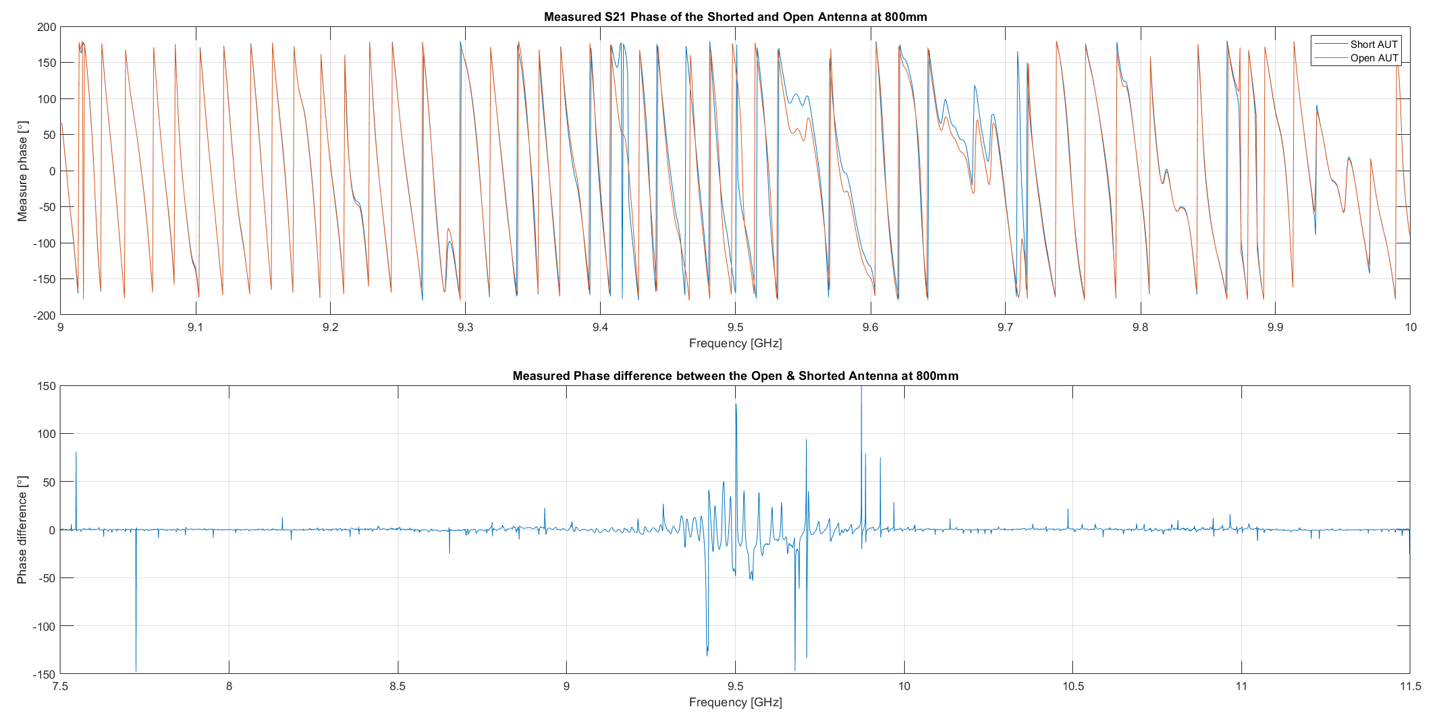
\includegraphics[width=0.99\linewidth]{Figures/chp4_Raw_difference_results.png}
    \caption{Measured and unprocessed phase difference between the open and short AUT.}
    \label{fig:chp4_Raw_difference_results}
    \end{figure}

Figure \ref{fig:chp4_Raw_smith} below shows the \(S_{21}\) at the center frequency plotted on the smith chart. Since the power loss from the transmit horn antenna through the test setup to the receive antenna is high, the magnitude of the \(S_{21}\) is very low. Due to this all three \(S_{21}\) points are difficult to see, figure \ref{fig:chp4_Raw_smith} (bottom) shows the same plot with a scale of 0.0032.

    \begin{figure}[H]
    \centering
    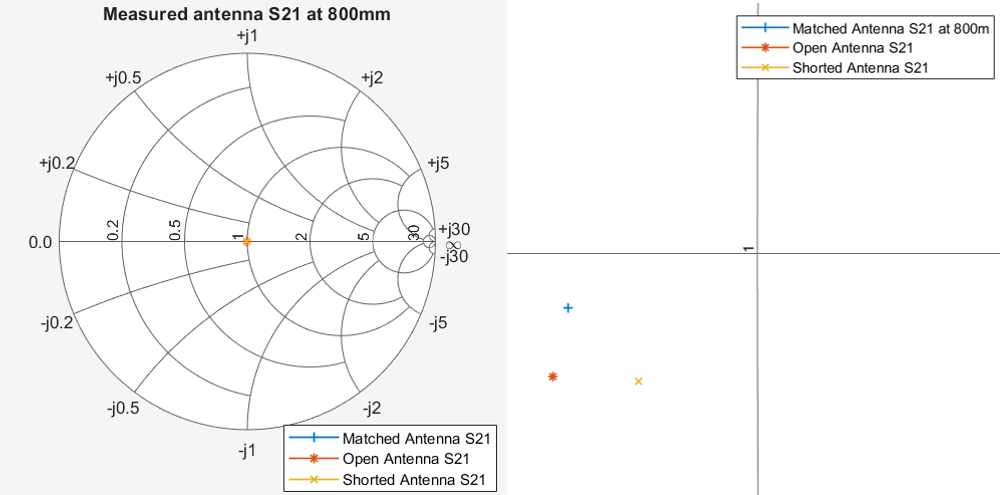
\includegraphics[width=0.9\linewidth]{Figures/chp4_Raw_smith.png}
    \caption{Measured and unprocessed \(S_{21}\) plotted on the smith chart.}
    \label{fig:chp4_Raw_smith}
    \end{figure}

For the proposed system in section \ref{sec:objectives}, it is assumed that the background and physical AUT remains constant for a given measurement. If that this assumption holds true, then the reflections received from the scene will be the same in the short circuit and open circuit measurement. Therefor this can be calibrated out. For the testing in this report the matched AUT should absorb all the received power into the 50$\Omega$ load and the received signal should only contain the reflections from the background and the physical structure of the AUT. Therefor all the measured \(S_{21}\) data is normalized to the matched \(S_{21}\) data as seen in figure \ref{fig:chp4_Calibrated_smith} below.

    \begin{figure}[H]
    \centering
    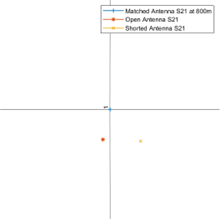
\includegraphics[width=0.4\linewidth]{Figures/chp4_Calibrated_smith.png}
    \caption{\(S_{21}\) normalized to the \(50\Omega S_{21}\) plotted on the smith chart.}
    \label{fig:chp4_Calibrated_smith}
    \end{figure}

Now that the short circuit and open circuit \(S_{21}\) has been normalized, the phase difference can be recalculated. Figure \ref{fig:chp4_Calibrated_difference_warpped_results} below shows the result over the entire measured frequency span. The spikes observed are due to the phase wrapping. Figure \ref{fig:chp4_Calibrated_difference_warpped_results}(bottom) show the result over the over the entire measured frequency span with the unwrapped phase.

    \begin{figure}[H]
    \centering
    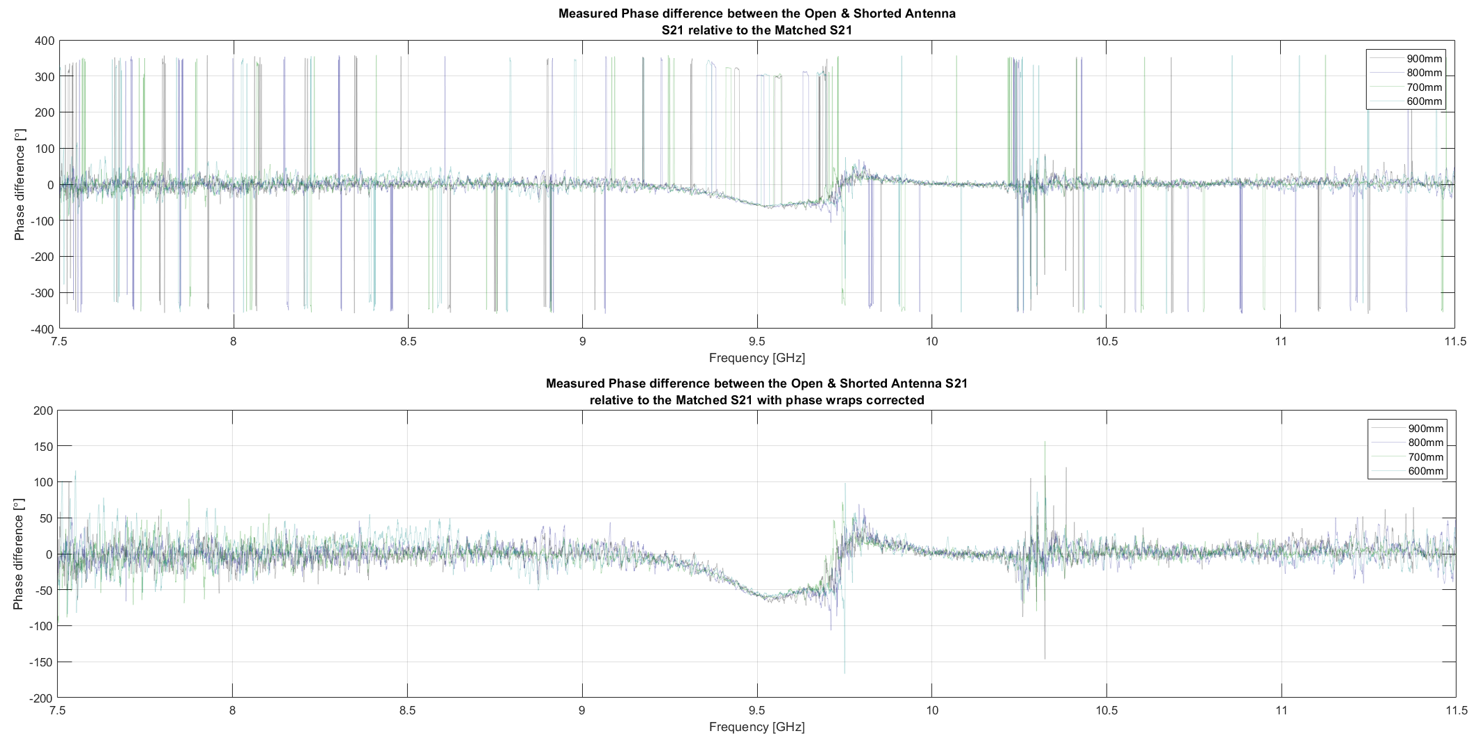
\includegraphics[width=0.9\linewidth]{Figures/chp4_Calibrated_difference_warpped_results.png}
    \caption{Encoded phase difference of the AUT normalized to the \(50\Omega \ S_{21}\).}
    \label{fig:chp4_Calibrated_difference_warpped_results}
    \end{figure}

It is undeniable that the phase difference becomes smaller the closer the measurement is to the center frequency. Figure \ref{fig:chp4_Calibrated_difference_zoom} below shows a zoomed-in plot of the phase difference. Using the antenna parameters as a guide the error calculations are done from 9.425-9.575GHz.

    \begin{figure}[H]
    \centering
    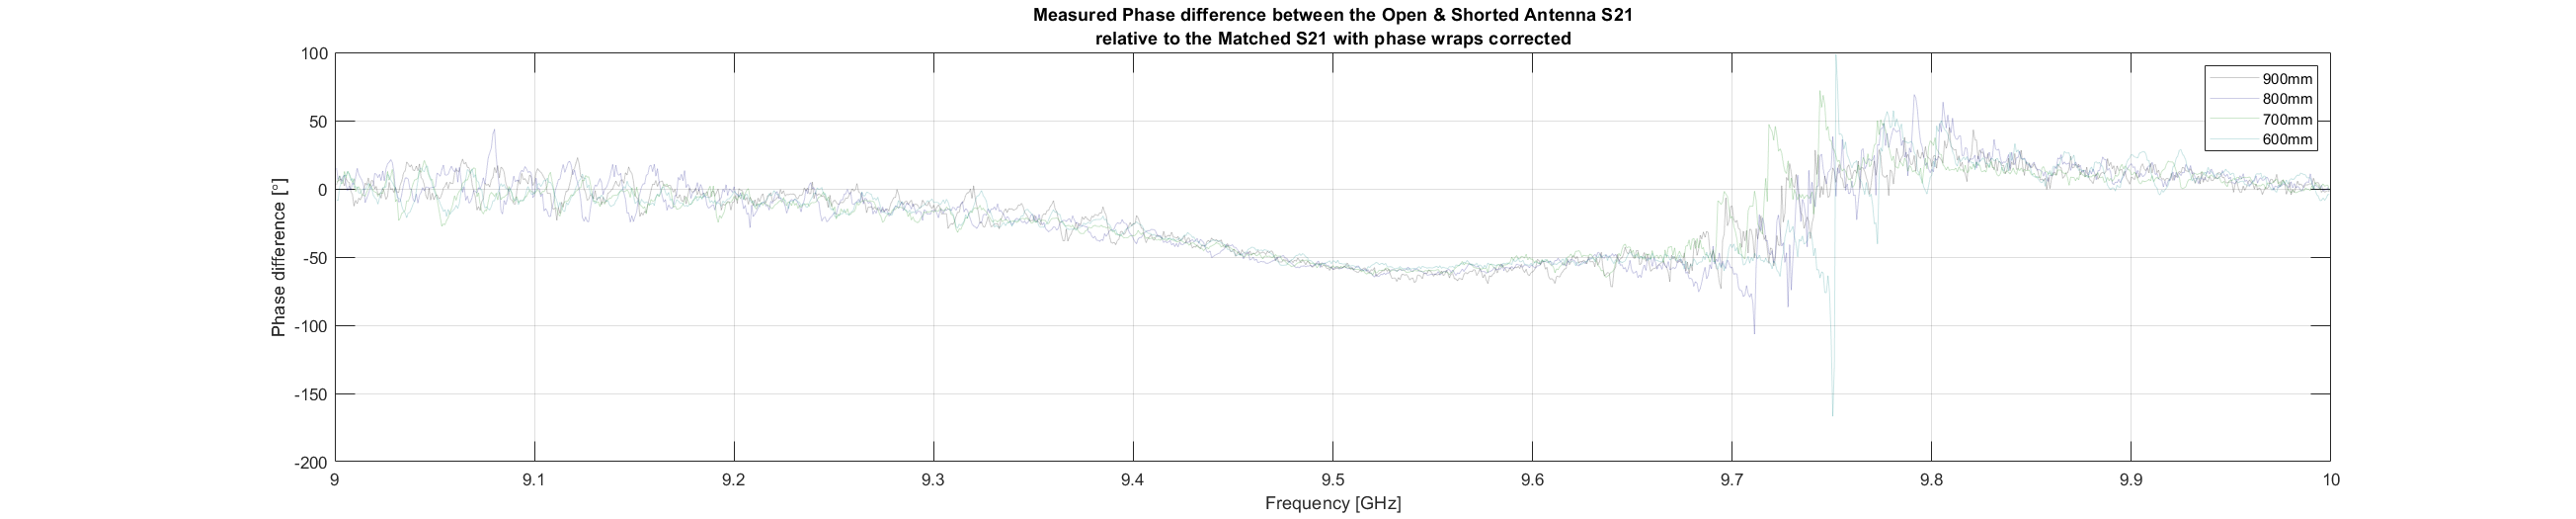
\includegraphics[width=0.99\linewidth]{Figures/chp4_Calibrated_difference_zoom.png}
    \caption{Zoomed-in plot of figure \ref{fig:chp4_Calibrated_difference_warpped_results}(bottom).}
    \label{fig:chp4_Calibrated_difference_zoom}
    \end{figure}

Figure \ref{fig:chp4_Calibrated_difference_results}(top) shows the mean of the four measurement sets over frequency along with the standard deviation from the mean over frequency (middle). The average of the mean is calculated as -53.71° and the average standard deviation is calculated as 2.66°. The phase error for each data set is seen in figure \ref{fig:chp4_Calibrated_difference_results}(bottom). The RMS phase error for each data set is noted in table \ref{tab:errorDay1}. These are very promising results, however the sample size is small and all four measurements set were recorded on the same say with the same environment. 

    \begin{table}[H]
    \centering
    \caption{Phase error of first set of measurements}
    \begin{tabular}{|l|r|} 
    \hline
    \textbf{Data set} & \textbf{RMS error [°]}   \\ 
    \hline
    900mm                 & 2.7193        \\ 
    \hline
    800mm                 & 2.7260     \\
    \hline
    700mm                 & 1.4218    \\
    \hline
    600mm                 & 2.9145     \\
    \hline
    \end{tabular}
    \label{tab:errorDay1}
    \end{table}

    \begin{figure}[H]
    \centering
    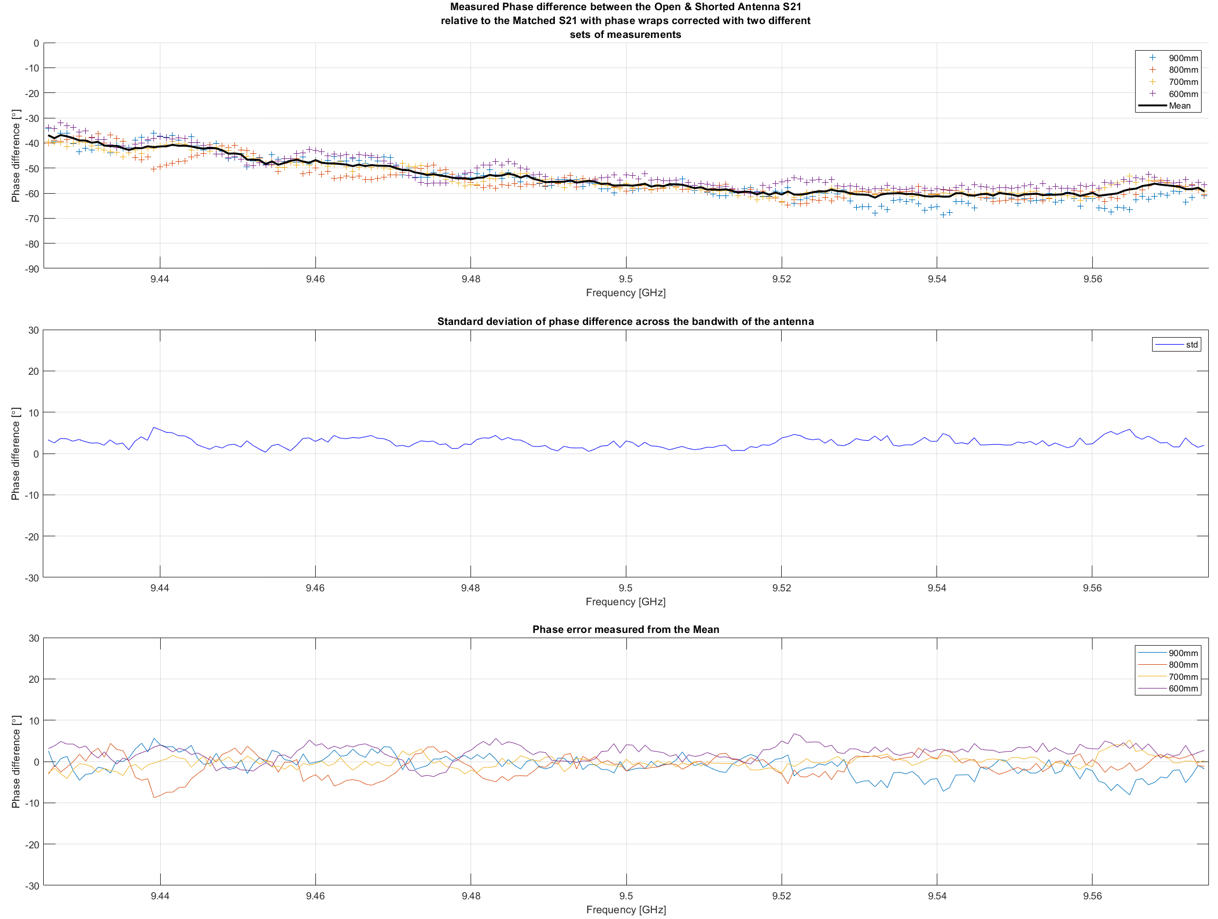
\includegraphics[width=0.99\linewidth]{Figures/chp4_Calibrated_difference_results.png}
    \caption{Mean, standard deviation and phase error of first set of measurements.}
    \label{fig:chp4_Calibrated_difference_results}
    \end{figure}

The tests are repeated two weeks after the original testing was completed to confirm that the results are correct and repeatable. Figure \ref{fig:chp4_Calibrated_smith_rept}(left) is from the first day of testing, figure \ref{fig:chp4_Calibrated_smith_rept}(right) is from the second day of testing. It is seen that the figure after normalizing to the \(50\Omega S_{21}\) the second measurement looks like a rotated version of the first measurement. The visual inspection is promising. 

    \begin{figure}[H]
    \centering
    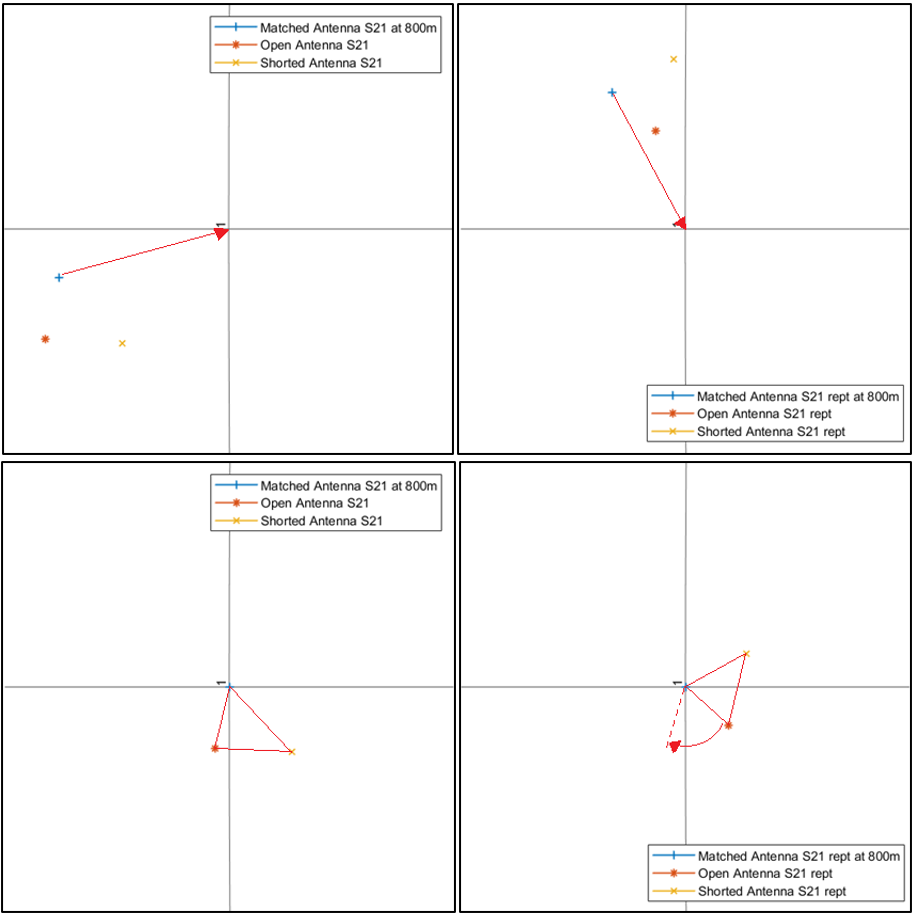
\includegraphics[width=0.9\linewidth]{Figures/chp4_Calibrated_smith_rept.png}
    \caption{First set \(S_{21}\) (left), Second set \(S_{21}\)(right).}
    \label{fig:chp4_Calibrated_smith_rept}
    \end{figure}

Figure \ref{fig:chp4_Calibrated_difference_rept_results} below shows the encoded phase difference between the short circuit and open circuit after being normalized to the matched \(S_{21}\). Figure  \ref{fig:chp4_Calibrated_difference_rept_results}(bottom) shows the same data overlayed over the first day of testing’s results. The response is similar, but slightly more sporadic.

    \begin{figure}[H]
    \centering
    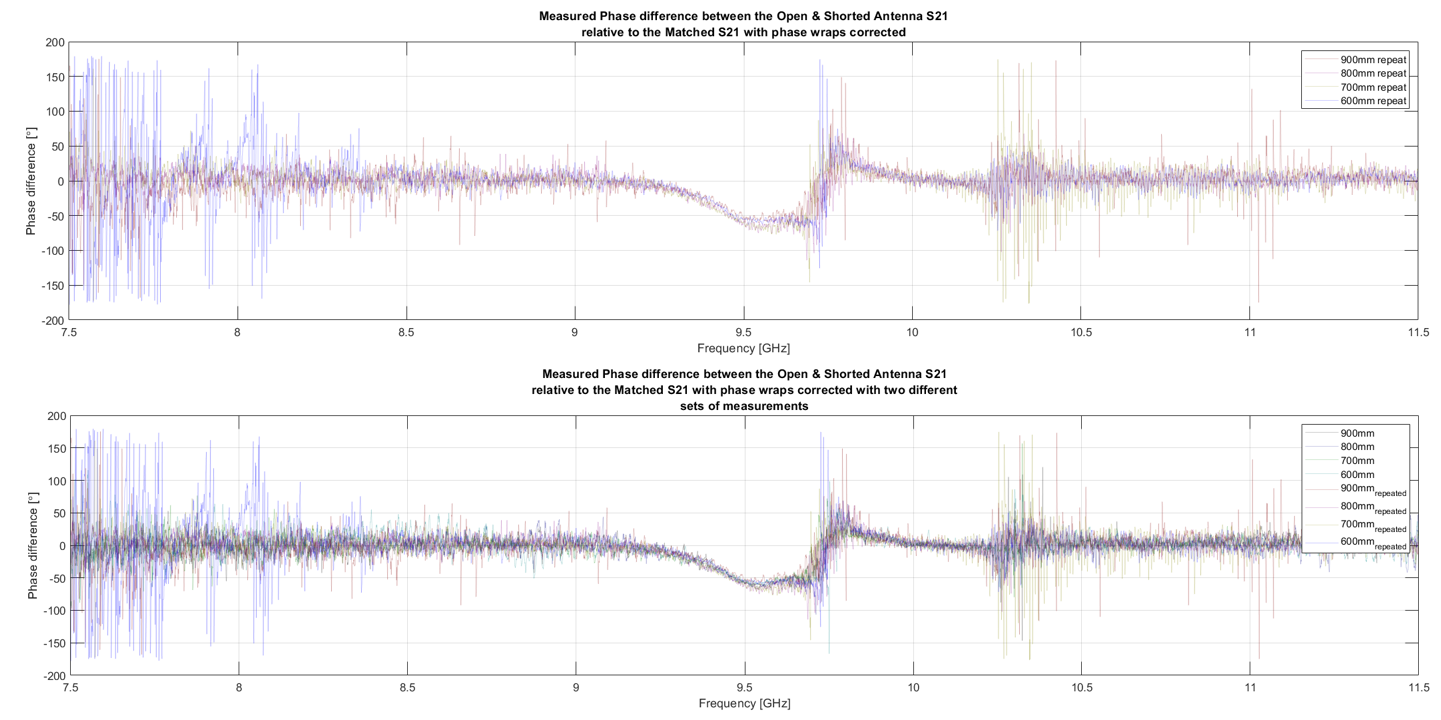
\includegraphics[width=0.99\linewidth]{Figures/chp4_Calibrated_difference_rept_results.png}
    \caption{Encoded phase difference of the AUT normalized to the \(50\Omega S_{21}\).}
    \label{fig:chp4_Calibrated_difference_rept_results}
    \end{figure}

Figure \ref{fig:chp4_Calibrated_difference_results_rept}(top) shows the recalculated mean of the all the measurement sets along with the recalculated and the original standard deviation from the mean (middle). The average of the mean is calculated as -54.06°, which is within 0.4° of the original mean. The average standard deviation is calculated as 4.19°, which has increased by 1.5° from the original standard deviation. The phase error for each data set is seen in figure \ref{fig:chp4_Calibrated_difference_results_rept}(bottom). The RMS phase error for each data set is noted in table \ref{tab:errorDay2} and a clear increase is observed.

    \begin{table}[H]
    \centering
    \caption{Phase error of all measurements}
    \begin{tabular}{|l|r|r|} 
    \hline
    \textbf{Data set} & \textbf{RMS error for day 1 [°]} & \textbf{RMS error for day 2 [°]}  \\ 
    \hline
    900mm                 & 2.7193    & 6.1314    \\ 
    \hline 
    800mm                 & 2.7260    & 5.0576 \\
    \hline
    700mm                 & 1.4218    & 5.2886  \\
    \hline
    600mm                 & 2.9145    & 3.1176  \\
    \hline
    \end{tabular}
    \label{tab:errorDay2}
    \end{table}

    \begin{figure}[H]
    \centering
    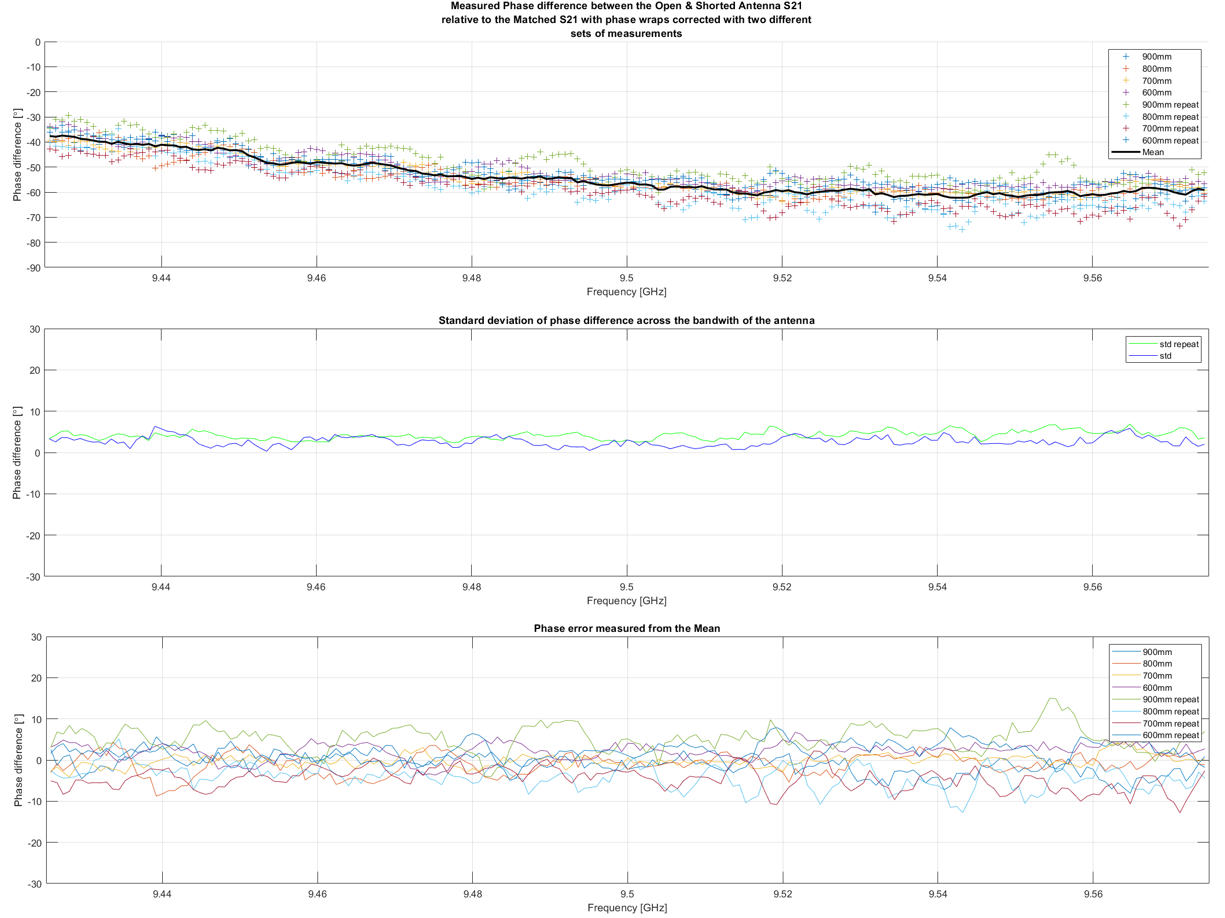
\includegraphics[width=0.99\linewidth]{Figures/chp4_Calibrated_difference_results_rept.png}
    \caption{Mean, standard deviation and phase error of all measurements.}
    \label{fig:chp4_Calibrated_difference_results_rept}
    \end{figure}

% ----------------------------------------------------
\ifstandalone
\bibliography{../Bibliography/References.bib}
\printnoidxglossary[type=\acronymtype,nonumberlist]
\fi
%\end{document}
% ----------------------------------------------------